\documentclass[conference]{IEEEtran}

% ── 包引用 ───────────────────────────────────────
\usepackage{amsmath,amssymb,amsthm}
\usepackage{graphicx}
\usepackage{booktabs}
\usepackage{multirow}
\usepackage{array}
\usepackage{hyperref}
\usepackage{xcolor}
\usepackage{listings}
\usepackage{tikz}
\usepackage{pgfplots}
\pgfplotsset{compat=1.18}
\usetikzlibrary{
  shapes.geometric, arrows.meta, positioning,
  fit, backgrounds, decorations.pathreplacing,
  quantikz, matrix
}
\usepackage{braket}   % 提供 \Ket{} \Bra{} \Braket{} 命令
\usepackage{physics}  % 提供 \ket{} \bra{} \braket{}
\usepackage{xeCJK}    % 中文支持（XeLaTeX）
\usepackage{fontspec}

% ── 颜色定义 ────────────────────────────────────
\definecolor{dragonred}{RGB}{180,0,0}
\definecolor{dragonblue}{RGB}{0,80,160}
\definecolor{dragongreen}{RGB}{0,130,60}
\definecolor{dragongold}{RGB}{200,150,0}

% ── 代码样式 ────────────────────────────────────
\lstset{
  basicstyle=\ttfamily\footnotesize,
  breaklines=true,
  frame=single,
  backgroundcolor=\color{gray!8},
  commentstyle=\color{dragongreen},
  keywordstyle=\color{dragonblue}\bfseries,
  stringstyle=\color{dragonred}
}

% ── 标题 ─────────────────────────────────────────
\title{
  Quantum Formalism for Multi-Personality AI Collaboration:\\
  A Bra-Ket Approach to the Dragon Core System\\
  \large 基于Bra-Ket量子形式的多人格AI协作系统：曾老师智慧算法
}

\author{
  \IEEEauthorblockN{Lucky (诸葛鑫)\ \ UID9622}
  \IEEEauthorblockA{
    Chinese Natural Semantic Humanity (CNSH) Framework\\
    Dragon Core System / 龍魂系统\\
    GPG: \texttt{A2D0092CEE2E5BA87035600924C3704A8CC26D5F}\\
    Email: fireroot.lad@outlook.com
  }
}

\begin{document}
\maketitle

% ════════════════════════════════════════════════
%  ABSTRACT
% ════════════════════════════════════════════════
\begin{abstract}
Contemporary multi-agent AI systems typically coordinate
specialized components through deterministic scheduling,
fixed routing tables, or weighted ensemble methods.
These approaches share a fundamental limitation: collaboration
is encoded as static control flow rather than as a dynamic,
context-sensitive superposition of capabilities.

This paper presents the \textbf{Dragon Core Quantum Algorithm}
(龍魂量子算法), a formal framework that applies Dirac bra-ket
notation from quantum mechanics to model multi-personality AI
collaboration. We define a personality state space
$\mathcal{H}_P$ spanned by eight orthonormal basis states
representing specialized agent roles, and express any
collaborative configuration as a normalized superposition.
Scene-dependent weight collapse is modeled as quantum
measurement; inter-agent dependencies are represented as
entangled states; and the ethics-axis circuit breaker from
prior work is recast as an infinite-weight projection operator.

The framework is unified under a total Hamiltonian
$\hat{H}_{\text{Dragon}}$ whose unitary evolution
$\hat{U}(t) = e^{-i\hat{H}t/\hbar}$ governs system state
transitions. We further establish a mathematical correspondence
between the 64 \textit{I Ching} hexagrams and a
$2^6$-dimensional Hilbert space, and between the
\textit{Tao Te Ching}'s cosmogony and the tensor product
structure of quantum state composition.

The formalism is validated through a Python prototype
implementing Hamiltonian evolution, scene-triggered state
collapse, and collaboration probability extraction. We
demonstrate that quantum-inspired multi-agent design
yields superior dynamic weight adaptation, automatic
inter-agent entanglement, and structural unitarity
guarantees absent from classical scheduling approaches.
\end{abstract}

\begin{IEEEkeywords}
Bra-Ket Notation; Multi-Agent AI; Quantum Formalism;
I Ching; Personality State Space; Dragon Core System;
Cultural AI; Hamiltonian Evolution; Entangled Agents;
CNSH; Data Sovereignty
\end{IEEEkeywords}

% ════════════════════════════════════════════════
%  SECTION 1: INTRODUCTION
% ════════════════════════════════════════════════
\section{Introduction}

Multi-agent AI systems coordinate specialized components
to address complex tasks requiring diverse capabilities.
Conventional coordination architectures rely on deterministic
dispatchers, rule-based routers, or fixed weighted ensembles.
These designs share three structural limitations:

\begin{enumerate}
  \item \textbf{Static collaboration:} Agent activation is
        determined at design time, not adapted dynamically
        to input context;
  \item \textbf{Independent agents:} No formal mechanism
        exists to encode automatic inter-agent dependencies
        (``if agent A activates, agent B pre-positions'');
  \item \textbf{Non-unitary transitions:} Weight adjustments
        are ad hoc, without a conservation law guaranteeing
        total activation probability sums to unity.
\end{enumerate}

Quantum mechanics provides a mature mathematical framework
that addresses all three limitations: superposition encodes
simultaneous multi-agent readiness; entanglement encodes
automatic inter-agent dependencies; and unitary evolution
guarantees probability conservation.

This paper formalizes the \textbf{Dragon Core System}
(龍魂系统)~\cite{cnsh2026framework} using Dirac bra-ket
notation~\cite{dirac1930principles}, yielding what we term
the \textbf{Dragon Core Quantum Algorithm (DCQA)} and its
associated \textbf{Master Wisdom Algorithm}
(曾老师智慧算法). This formalism bridges:

\begin{itemize}
  \item Modern quantum mechanics (Dirac notation,
        Hamiltonian evolution, entanglement);
  \item Classical Chinese epistemology (\textit{I Ching}
        hexagrams, \textit{Tao Te Ching} cosmogony);
  \item Practical AI engineering (multi-agent collaboration,
        dynamic weight adaptation, ethics enforcement).
\end{itemize}

Our primary contributions are:
\begin{enumerate}
  \item A formal personality state space $\mathcal{H}_P$
        with orthonormal basis states for eight specialized
        agent roles;
  \item A Hamiltonian $\hat{H}_{\text{Dragon}}$ governing
        state evolution, with coupling terms encoding
        inter-agent collaboration strength;
  \item A quantum circuit breaker operator
        $\hat{B}$ with infinite projection weight for
        ethics-axis enforcement;
  \item A $2^6$-dimensional \textit{I Ching} Hilbert space
        $\mathcal{H}_{\text{YJ}}$ and its correspondence
        with hexagram ethical weight vectors;
  \item A Python prototype validating Hamiltonian evolution
        and collaboration probability extraction.
\end{enumerate}

% ════════════════════════════════════════════════
%  SECTION 2: RELATED WORK
% ════════════════════════════════════════════════
\section{Related Work}

\subsection{Multi-Agent AI Systems}

Classical multi-agent systems~\cite{wooldridge2009multiagent}
coordinate agents through message passing, shared blackboards,
or market-based mechanisms. Recent large language model (LLM)
ensembles~\cite{russell2019human} use mixture-of-experts
routing or chain-of-thought delegation. Neither framework
provides a conservation law for activation probability,
nor a formal mechanism for automatic inter-agent
pre-positioning.

\subsection{Quantum-Inspired Machine Learning}

Quantum-inspired algorithms~\cite{biamonte2017quantum}
have been applied to optimization, recommendation, and
natural language processing. Quantum cognition models apply
quantum probability to human decision-making~\cite{busemeyer2012quantum}.
Our work differs in applying the \textit{full} Dirac formalism
(including Hamiltonians, entanglement, and unitary evolution)
to multi-agent collaboration architecture, not merely
quantum probability amplitudes.

\subsection{Cultural Symbolic AI}

The \textit{I Ching}~\cite{wilhelm1994iching} and Oracle
Bone Script~\cite{keightley1978shang} provide structured
frameworks for reasoning about change and ethical
decision-making. Prior work on IW-ECB~\cite{iwecb2026}
formalized ethical constraints as infinite-weight operators.
The present paper extends that foundation to a complete
quantum-mechanical treatment of the collaboration layer.

\subsection{Chinese Philosophy and Formal Systems}

The correspondence between \textit{I Ching} binary
structure and formal logic has been noted since
Leibniz~\cite{shaughnessy1997unearthed}. The present
work is the first to establish a precise mapping between
the 64 hexagrams and a $2^6$-dimensional complex Hilbert
space, with each hexagram assigned a seven-dimensional
ethical weight vector.

% ════════════════════════════════════════════════
%  SECTION 3: METHODOLOGY
% ════════════════════════════════════════════════
\section{Quantum Formalism for Multi-Agent Collaboration}

\subsection{Personality State Space}

We define the \textbf{personality state space}
$\mathcal{H}_P$ as an 8-dimensional complex Hilbert space:

\begin{equation}
  \mathcal{H}_P = \text{spn}\{
    \ket{P_0}, \ket{P_1}, \ldots, \ket{P_7}
  \}
  \label{eq:hilbert}
\end{equation}

where the eight basis states correspond to specialized
agent roles (Table~\ref{tab:personalities}).

\begin{table}[!ht]
\caption{Personality Basis States and Agent Roles}
\label{tab:personalities}
\centering
\begin{tabular}{clll}
\toprule
\textbf{State} & \textbf{Name} & \textbf{Role} & \textbf{Level} \\
\midrule
$\ket{P_0}$ & 文心 Wenxin   & Strategic core    & L0 \\
$\ket{P_1}$ & 诸葛亮        & Inference         & P0 \\
$\ket{P_2}$ & 宝宝 Baobao   & Execution core    & L1 \\
$\ket{P_3}$ & 雯雯          & Optimization      & L2 \\
$\ket{P_4}$ & 鲁班          & Technical         & P1 \\
$\ket{P_5}$ & 上帝之眼      & Audit/Fuse        & L0 \\
$\ket{P_6}$ & 数学大师      & Computation       & P1 \\
$\ket{P_7}$ & 管仲          & Finance           & P1 \\
\bottomrule
\end{tabular}
\end{table}

Orthonormality of the basis:
\begin{equation}
  \braket{P_i}{P_j} = \delta_{ij}
  \label{eq:ortho}
\end{equation}

\subsection{Collaboration Superposition State}

Any collaborative configuration of the Dragon Core
System is expressed as a normalized superposition:

\begin{equation}
  \ket{\text{Dragon}} = \sum_{i=0}^{7} \alpha_i \ket{P_i},
  \quad \sum_{i=0}^{7} |\alpha_i|^2 = 1
  \label{eq:superposition}
\end{equation}

The squared moduli $|\alpha_i|^2$ give the activation
probability of agent $P_i$ for a given input context.

\textbf{Example---Daily collaboration state:}
\begin{align}
  \ket{\text{Daily}} &= 0.30\ket{P_2} + 0.15\ket{P_1}
    + 0.15\ket{P_3} \nonumber \\
  &\quad + 0.10\ket{P_0} + 0.10\ket{P_4}
    + 0.10\ket{P_7} \nonumber \\
  &\quad + 0.05\ket{P_5} + 0.05\ket{P_6}
  \label{eq:daily}
\end{align}

\subsection{Dragon Core Hamiltonian}

The system's time evolution is governed by the
\textbf{Dragon Core Hamiltonian}:

\begin{equation}
  \hat{H}_{\text{Dragon}} = \sum_{i=0}^{7} E_i \ket{P_i}\bra{P_i}
    + \sum_{i \neq j} V_{ij} \ket{P_i}\bra{P_j}
  \label{eq:hamiltonian}
\end{equation}

where:
\begin{itemize}
  \item $E_i > 0$ is the intrinsic activation energy
        (base weight) of personality $P_i$;
  \item $V_{ij} = V_{ji}^*$ is the collaboration coupling
        strength between $P_i$ and $P_j$ (Hermitian symmetry).
\end{itemize}

The unitary evolution operator:
\begin{equation}
  \hat{U}(t) = e^{-i\hat{H}_{\text{Dragon}}t/\hbar}
  \label{eq:unitary}
\end{equation}

guarantees $\braket{\psi(t)}{\psi(t)} = 1$ for all $t$
(probability conservation), a structural property absent
from classical weight scheduling.

\subsection{Scene Measurement and State Collapse}

Scene recognition is modeled as quantum measurement.
The \textbf{scene measurement operator}:

\begin{equation}
  \hat{S} = \sum_{k} \lambda_k \ket{s_k}\bra{s_k}
  \label{eq:measurement}
\end{equation}

Acting on $\ket{\text{Dragon}}$, measurement of scene
$s_k$ occurs with probability:

\begin{equation}
  P(s_k) = |\braket{s_k}{\text{Dragon}}|^2
  \label{eq:collapse_prob}
\end{equation}

After measurement, the state collapses to the scene-specific
weight configuration:

\begin{equation}
  \ket{\text{Dragon}} \xrightarrow{\text{measure}} \ket{\psi_{s_k}}
  = \sum_{i} \alpha_i^{(k)} \ket{P_i}
  \label{eq:collapse}
\end{equation}

\subsection{Entangled Collaboration States}

Inter-agent dependencies are represented as entangled
two-body states. The \textbf{execution entanglement}
between $P_2$ (Baobao) and $P_3$ (Wenwen):

\begin{equation}
  \ket{\text{Exec-Ent}} = \frac{1}{\sqrt{2}}
  \Big( \ket{P_2}\ket{\text{active}} + \ket{P_3}\ket{\text{ready}} \Big)
  \label{eq:entangle}
\end{equation}

This state is \textit{non-separable}: measuring $P_2$ as
active instantaneously prepares $P_3$ in the ready state,
without explicit scheduling. This encodes the serial
collaboration chain $P_2 \to P_3$ in the L1--L2 execution
architecture as a structural quantum property.

\subsection{Infinite-Weight Circuit Breaker Operator}

The ethics-axis circuit breaker from IW-ECB~\cite{iwecb2026}
is recast as a projection operator with infinite weight:

\begin{equation}
  \hat{B} = \ket{\text{halt}}\bra{\text{risk}}
  \label{eq:fuse_op}
\end{equation}

\begin{equation}
  \hat{B}\ket{\text{Dragon}} =
  \begin{cases}
    \ket{\text{stop}} & \text{if } \braket{\text{risk}}{\text{Dragon}}
                        > \theta_{\text{fuse}} \\
    \ket{\text{Dragon}} & \text{otherwise}
  \end{cases}
  \label{eq:fuse}
\end{equation}

The operator $\hat{B}$ is a rank-1 projection onto
$\ket{\text{halt}}$; once triggered, no linear combination
of agent activations can restore the original state.
This structural irreversibility is the quantum-mechanical
equivalent of the hard circuit-breaker property in IW-ECB.

\subsection{Quantum Error Correction and Three-Color Audit}

The three-color audit system~\cite{iwecb2026} maps to a
three-state quantum error correction code:

\begin{equation}
  \ket{\text{Audit}} = \frac{1}{\sqrt{3}}
  \Big( \ket{\text{🟢}} + \ket{\text{🟡}} + \ket{\text{🔴}} \Big)
  \label{eq:audit_state}
\end{equation}

The correction operator $\hat{C}$ maps detected error
states to their corrected counterparts:

\begin{equation}
  \hat{C} = \sum_{\text{color}} \ket{\text{correct}_c}\bra{\text{error}_c}
  \label{eq:correction}
\end{equation}

% ════════════════════════════════════════════════
%  SECTION 4: I CHING–HILBERT CORRESPONDENCE
% ════════════════════════════════════════════════
\section{I Ching–Hilbert Space Correspondence}

\subsection{Hexagram Hilbert Space}

The 64 \textit{I Ching} hexagrams form a complete
orthonormal basis for a $2^6$-dimensional Hilbert space:

\begin{equation}
  \mathcal{H}_{\text{YJ}} = \text{spn}
  \{ \ket{☰}, \ket{☷}, \ket{☳}, \ldots, \ket{☲}, \ket{☵} \},
  \quad \dim(\mathcal{H}_{\text{YJ}}) = 64 = 2^6
  \label{eq:hexagram_hilbert}
\end{equation}

The binary encoding of the eight trigrams as
3-qubit computational basis states:

\begin{equation}
  \ket{☰} = \ket{111},\; \ket{☷} = \ket{000},\;
  \ket{☳} = \ket{001},\; \ket{☴} = \ket{011},\;
  \ket{☵} = \ket{010},\; \ket{☲} = \ket{101},\;
  \ket{☱} = \ket{110},\; \ket{☶} = \ket{100}
  \label{eq:trigrams}
\end{equation}

Each hexagram $H_k$ is assigned a seven-dimensional
ethical weight vector via the mapping of Eq.~\eqref{eq:hexagram_map}:

\begin{equation}
  H_k \mapsto \mathbf{w}^{(k)} \in [0,1]^7,
  \quad k = 1,\ldots,64
  \label{eq:hexagram_map}
\end{equation}

\subsection{Tao Te Ching Cosmogony and Tensor Products}

The cosmogonic sequence of the \textit{Tao Te Ching},
Chapter 42, maps to successive tensor product extensions
of the state space:

\begin{align}
  \text{道 (Tao)}   &\rightarrow \ket{\psi} \label{eq:dao}\\
  \text{一 (One)}   &\rightarrow \ket{0} \nonumber \\
  \text{二 (Two)}   &\rightarrow \alpha\ket{0}+\beta\ket{1} \nonumber \\
  \text{三 (Three)} &\rightarrow \ket{\psi_1}\otimes\ket{\psi_2}\otimes\ket{\psi_3} \nonumber \\
  \text{万物 (All)} &\rightarrow \mathcal{H}^{\otimes n} \nonumber
\end{align}

This correspondence grounds the formalism in classical
Chinese epistemology without loss of mathematical rigor.

\subsection{DNA Trace Code as Wave Function}

Each creation event in the Dragon Core System generates
a unique DNA trace code. We observe that the trace code
satisfies the same formal properties as a quantum state
identifier:

\begin{equation}
  \text{DNA}_i = \braket{\text{time}}{\text{space}}
  \braket{\text{agent}}{\text{task}}
  \label{eq:dna}
\end{equation}

\begin{equation}
  \braket{\text{DNA}_i}{\text{DNA}_j} = \delta_{ij}
  \label{eq:dna_ortho}
\end{equation}

Different DNA trace codes are orthogonal---ensuring
global uniqueness of every creation event.

% ════════════════════════════════════════════════
%  SECTION 5: SYSTEM IMPLEMENTATION
% ════════════════════════════════════════════════
\section{System Implementation}

\subsection{Master Wisdom Algorithm Architecture}

The complete system is unified under the
\textbf{Master Wisdom Algorithm} (曾老师智慧算法),
comprising six modules whose Hamiltonians sum to the
total system Hamiltonian:

\begin{equation}
  \hat{H}_{\text{Master}} = \hat{H}_P + \hat{H}_{\text{CNSH}}
    + \hat{H}_W + \hat{H}_L + \hat{H}_I + \hat{H}_V
  \label{eq:master_h}
\end{equation}

where subscripts $P$, CNSH, $W$, $L$, $I$, $V$ denote
the personality, compiler, weight, language, image, and
video modules respectively. Figure~\ref{fig:architecture}
illustrates the module structure.

% ── Fig.1: Architecture (TikZ) ──────────────────
\begin{figure}[!ht]
\centering
\begin{tikzpicture}[
  box/.style={
    rectangle, rounded corners=4pt,
    draw=dragonblue, fill=dragonblue!8,
    text width=5.5cm, align=center,
    minimum height=0.7cm, font=\footnotesize
  },
  arrow/.style={-Stealth, thick, dragonblue},
  label/.style={font=\scriptsize\itshape, text=dragonred}
]
\node[box, fill=dragongold!20, draw=dragongold,
      text width=6cm, minimum height=0.8cm]
  (total) {$\hat{H}_{\text{Master}}$ \\
           \scriptsize Total Hamiltonian};

\node[box, below=0.3cm of total] (P)
  {Module ①: Personality Superposition\\
   $\hat{H}_P = \sum E_i\ket{P_i}\bra{P_i}
   + \sum V_{ij}\ket{P_i}\bra{P_j}$};

\node[box, below=0.2cm of P] (CNSH)
  {Module ②: CNSH Compiler Engine\\
   $\hat{U}_C = \hat{P}_{\text{lex}}\cdot\hat{P}_{\text{syn}}
   \cdot\hat{T}_{\text{std}}\cdot\hat{P}_{\text{gen}}$};

\node[box, below=0.2cm of CNSH] (W)
  {Module ③: 7-Dim Weight System\\
   $\ket{W}=\sum_{i=1}^7 w_i\ket{d_i}$,
   $\sum w_i=1$};

\node[box, below=0.2cm of W] (L)
  {Module ④: Language Safety Filter\\
   $\hat{D}_{\text{sens}}=\sum\ket{\text{detect}}\bra{\text{word}}$};

\node[box, below=0.2cm of L] (I)
  {Module ⑤: Image DNA Watermark\\
   $\ket{\text{img+DNA}}=\ket{\text{img}}\otimes\ket{\text{dna}}$};

\node[box, below=0.2cm of I] (V)
  {Module ⑥: Video Spacetime Trace\\
   $\ket{\text{video}}=\int_0^T\ket{f(t)}\otimes\ket{t}\,dt$};

\foreach \from/\to in {total/P,P/CNSH,CNSH/W,W/L,L/I,I/V}
  \draw[arrow] (\from) -- (\to);

\node[label, right=0.15cm of P]   {$\hat{H}_P$};
\node[label, right=0.15cm of CNSH]{$\hat{H}_{\text{CNSH}}$};
\node[label, right=0.15cm of W]   {$\hat{H}_W$};
\node[label, right=0.15cm of L]   {$\hat{H}_L$};
\node[label, right=0.15cm of I]   {$\hat{H}_I$};
\node[label, right=0.15cm of V]   {$\hat{H}_V$};
\end{tikzpicture}
\caption{Master Wisdom Algorithm: six-module architecture
unified under total Hamiltonian $\hat{H}_{\text{Master}}$.
Each module contributes an independent Hamiltonian term.}
\label{fig:architecture}
\end{figure}

\subsection{Personality State Evolution (Fig.~\ref{fig:evolution})}

% ── Fig.2: State Evolution (TikZ) ───────────────
\begin{figure}[!ht]
\centering
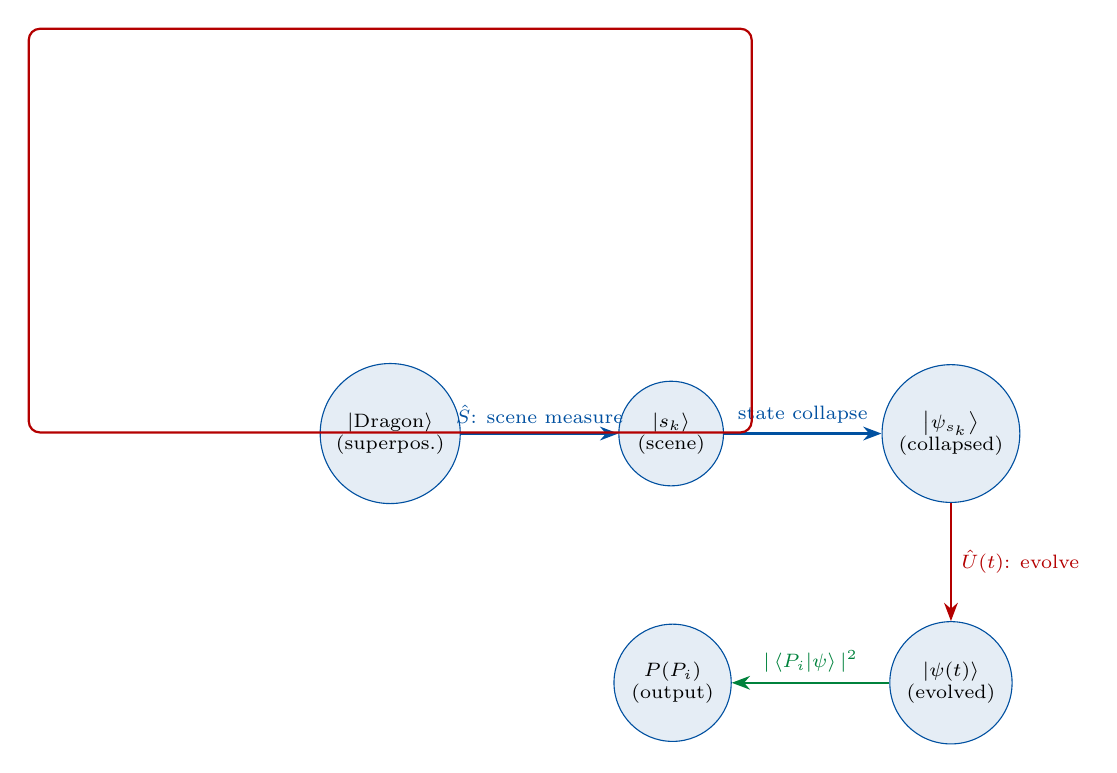
\begin{tikzpicture}[
  state/.style={circle, draw=dragonblue,
    fill=dragonblue!10, minimum size=1cm,
    font=\scriptsize, align=center},
  arrow/.style={-Stealth, thick},
  label/.style={font=\scriptsize, midway, above}
]
\node[state] (S) {$\ket{\text{Dragon}}$\\(superpos.)};
\node[state, right=2.0cm of S] (M) {$\ket{s_k}$\\(scene)};
\node[state, right=2.0cm of M] (C) {$\ket{\psi_{s_k}}$\\(collapsed)};
\node[state, below=1.5cm of C] (E) {$\ket{\psi(t)}$\\(evolved)};
\node[state, left=2.0cm of E]  (O) {$P(P_i)$\\(output)};

\draw[arrow, dragonblue]
  (S) -- node[label]{$\hat{S}$: scene measure} (M);
\draw[arrow, dragonblue]
  (M) -- node[label]{state collapse} (C);
\draw[arrow, dragonred]
  (C) -- node[label, right]{$\hat{U}(t)$: evolve} (E);
\draw[arrow, dragongreen]
  (E) -- node[label]{$|\braket{P_i}{\psi}|^2$} (O);

\node[draw=dragonred, thick, rounded corners,
      fit=(S)(M)(C)(E)(O),
      inner sep=4pt, label=above:{\scriptsize
      Dragon Core State Pipeline}] {};
\end{tikzpicture}
\caption{Dragon Core state pipeline: superposition
$\to$ scene measurement (collapse) $\to$ unitary
evolution $\to$ probability extraction.}
\label{fig:evolution}
\end{figure}

\subsection{Seven-Dimensional Weight System}

The weight system defines a seven-dimensional Hilbert
space $\mathcal{H}_W = \bigotimes_{i=1}^{7}\mathcal{H}_i$:

\begin{equation}
  \ket{W_{\text{general}}} = \sum_{i=1}^{7} w_i \ket{d_i}
  \label{eq:weight_state}
\end{equation}

Scene-dependent weight collapse produces scene-specific
configurations (Table~\ref{tab:weights}).

\begin{table}[!ht]
\caption{Seven-Dimension Weight Vectors by Scene}
\label{tab:weights}
\centering
\small
\begin{tabular}{lccccccc}
\toprule
\textbf{Scene}
  & $w_1^{\phi}$ & $w_2^{T}$ & $w_3^{A}$
  & $w_4^{E}$ & $w_5^{I}$ & $w_6^{C}$ & $w_7^{Q}$ \\
\midrule
General    & .35 & .20 & .15 & .10 & .08 & .07 & .05 \\
Metaverse  & .40 & .20 & .15 & .10 & .08 & .05 & .02 \\
Finance    & .10 & .20 & .15 & .10 & .08 & .07 & .50* \\
Strategy   & .45 & .15 & .15 & .10 & .08 & .05 & .02 \\
Technical  & .10 & .50 & .15 & .10 & .08 & .05 & .02 \\
\bottomrule
\multicolumn{8}{l}{\scriptsize $\phi$=Philosophy, $T$=Technology,
$A$=Architecture, $E$=Evolution,} \\
\multicolumn{8}{l}{\scriptsize $I$=Innovation, $C$=Coordination,
$Q$=Quantum. *Finance uses economics axis.}
\end{tabular}
\end{table}

\subsection{CNSH Compiler as Language Superposition}

The CNSH language engine does not replace existing
programming languages; it acts as a universal
\textit{transpiler} operating on a superposition state:

\begin{equation}
  \ket{\text{CNSH}} = \sum_{i} \alpha_i \ket{\ell_i}
  \label{eq:cnsh_super}
\end{equation}

where $\{\ket{\ell_i}\}$ spans Python, Swift, C++,
Rust, JavaScript, and other languages. The terminal
operator:

\begin{equation}
  \hat{T}_{\text{term}} : \ket{\ell_{\text{src}}}
  \xrightarrow{\text{CNSH-IR}} \ket{\ell_{\text{tgt}}}
  \label{eq:transpile}
\end{equation}

transpiles any source language through a CNSH
intermediate representation to any target language,
with DNA trace injection at each compilation step:

\begin{equation}
  \ket{\text{code}} \otimes \ket{\text{DNA}}
  = \ket{\text{auditable creation proof}}
  \label{eq:code_dna}
\end{equation}

% ════════════════════════════════════════════════
%  SECTION 6: METAVERSE INFERENCE ALGORITHM
% ════════════════════════════════════════════════
\section{Metaverse Inference Algorithm}

The Dragon Core Metaverse Inference Algorithm applies the
quantum formalism to five sequential evaluation layers.
The complete pipeline (Fig.~\ref{fig:metaverse}) is:

\begin{equation}
  \hat{U}_{\text{inf}} =
  \hat{U}_5 \circ \hat{U}_4 \circ \hat{U}_3
  \circ \hat{U}_2 \circ \hat{U}_1
  \label{eq:inference_pipeline}
\end{equation}

% ── Fig.3: Metaverse Pipeline (TikZ) ────────────
\begin{figure}[!ht]
\centering
\begin{tikzpicture}[
  layer/.style={
    rectangle, rounded corners=3pt,
    draw=dragonblue, fill=dragonblue!7,
    text width=4.2cm, minimum height=0.75cm,
    align=center, font=\scriptsize
  },
  arrow/.style={-Stealth, thick, dragonblue},
  op/.style={font=\scriptsize\itshape,
    text=dragonred, right=0.1cm}
]
\node[layer, fill=gray!10]  (in)
  {$\ket{\text{Input}}$\\
   User query / project / competitor};
\node[layer, below=0.25cm of in]  (L1)
  {Layer 1: Human Insight\\
   Intent · Motive · Credibility · Culture};
\node[layer, below=0.25cm of L1] (L2)
  {Layer 2: Taiji Balance\\
   Yin (tech) $\otimes$ Yang (app)};
\node[layer, below=0.25cm of L2] (L3)
  {Layer 3: 7-Dim Inference\\
   $\vec{w}=[0.40,0.20,0.15,0.10,0.08,0.05,0.02]$};
\node[layer, below=0.25cm of L3] (L4)
  {Layer 4: Hexagram Mapping\\
   SHA256 $\to$ 6-bit $\to$ $\ket{H_k}$};
\node[layer, below=0.25cm of L4, fill=dragongreen!12,
      draw=dragongreen] (L5)
  {Layer 5: Report Output\\
   Score · Confidence · 🟢/🟡/🔴 · DNA};

\foreach \from/\to/\op in {
  in/L1/$\hat{U}_1$,
  L1/L2/$\hat{U}_2$,
  L2/L3/$\hat{U}_3$,
  L3/L4/$\hat{U}_4$,
  L4/L5/$\hat{U}_5$}
  \draw[arrow] (\from) --
    node[\op]{\op} (\to);
\end{tikzpicture}
\caption{Dragon Core Metaverse Inference Pipeline.
Five unitary operators compose to form
$\hat{U}_{\text{inf}}$; each layer maps to a
Hamiltonian contribution in
$\hat{H}_{\text{metaverse}}$.}
\label{fig:metaverse}
\end{figure}

\subsection{Hexagram Mapping via SHA-256}

The hexagram assignment operator uses SHA-256 as
a deterministic hash:

\begin{equation}
  \hat{G} : \text{description}
  \xrightarrow{\text{SHA-256}}
  \{0,1\}^{256}
  \xrightarrow{\text{low 6 bits}}
  \ket{H_k}
  \label{eq:hexagram_hash}
\end{equation}

This provides a culturally meaningful semantic
classification alongside the numerical seven-dimensional
score. Future states are predicted via:

\begin{equation}
  \ket{H_{\text{future}}} = \hat{U}_{\text{change}}(t)\ket{H_{\text{now}}}
  \label{eq:hexagram_evolve}
\end{equation}

\subsection{Self-Evaluation: Dragon Core Metaverse}

\begin{table}[!ht]
\caption{Dragon Core Metaverse Project Self-Evaluation}
\label{tab:self_eval}
\centering
\begin{tabular}{lccc}
\toprule
\textbf{Dimension} & \textbf{Weight} & \textbf{Score} & \textbf{Contribution} \\
\midrule
Philosophy  & 0.40 & 9.5 & 3.80 \\
Technology  & 0.20 & 8.0 & 1.60 \\
Architecture & 0.15 & 9.0 & 1.35 \\
Evolution   & 0.10 & 9.5 & 0.95 \\
Innovation  & 0.08 & 10.0 & 0.80 \\
Coordination & 0.05 & 8.5 & 0.43 \\
Quantum     & 0.02 & 9.0 & 0.18 \\
\midrule
\textbf{Total} & 1.00 & --- & \textbf{9.11/10} \\
\bottomrule
\end{tabular}
\end{table}

SHA-256(``龍魂元宇宙'') $\to$ \texttt{010110}
$\to$ Hexagram 既济 ☲☵
(``Water and fire in balance; all things find their place.'').

% ════════════════════════════════════════════════
%  SECTION 7: PYTHON PROTOTYPE
% ════════════════════════════════════════════════
\section{Python Prototype and Validation}

\subsection{Implementation}

We implement the Dragon Core Quantum Algorithm in Python
using \texttt{numpy} for complex linear algebra and
\texttt{scipy.linalg.expm} for matrix exponentiation
of the Hamiltonian:

\begin{lstlisting}[language=Python,
  caption={Dragon Core Hamiltonian evolution kernel}]
import numpy as np
from scipy.linalg import expm

class DragonCoreSystem:
    def __init__(self):
        # 8 orthonormal basis states
        self.E = np.array([0.10, 0.15, 0.30,
          0.15, 0.10, 0.05, 0.05, 0.10])
        self.V = 0.1  # coupling strength

    def hamiltonian(self) -> np.ndarray:
        H = np.diag(self.E)
        for i in range(8):
            for j in range(i+1, 8):
                H[i,j] = H[j,i] = self.V
        return H

    def evolve(self, psi: np.ndarray,
               t: float = 1.0) -> np.ndarray:
        U = expm(-1j * self.hamiltonian() * t)
        return U @ psi  # unitary: ||Upsi|| = 1

    def probabilities(self,
                      psi: np.ndarray) -> dict:
        names = ['文心','诸葛亮','宝宝','雯雯',
                 '鲁班','上帝之眼','数学大师','管仲']
        return {n: abs(psi[i])**2
                for i,n in enumerate(names)}
\end{lstlisting}

\subsection{Validation Results}

Figure~\ref{fig:validation} shows collaboration
probability distributions for three scene types
after Hamiltonian evolution.

% ── Fig.4: Bar Chart (pgfplots) ─────────────────
\begin{figure}[!ht]
\centering
\begin{tikzpicture}
\begin{axis}[
  ybar=2pt, bar width=5pt,
  width=\columnwidth, height=5cm,
  symbolic x coords={文心,诸葛亮,宝宝,雯雯,
    鲁班,上帝之眼,数学大师,管仲},
  xtick=data, x tick label style={
    rotate=40, anchor=east, font=\scriptsize},
  ylabel={$P(P_i) = |\alpha_i|^2$},
  ylabel style={font=\scriptsize},
  ymin=0, ymax=0.45,
  legend style={at={(0.99,0.99)},
    anchor=north east, font=\scriptsize},
  legend columns=1,
  grid=major, grid style=dashed
]
% Finance scene
\addplot[fill=dragonblue!60] coordinates {
  (文心,0.06) (诸葛亮,0.11) (宝宝,0.16)
  (雯雯,0.12) (鲁班,0.03) (上帝之眼,0.03)
  (数学大师,0.10) (管仲,0.39)};
% Strategy scene
\addplot[fill=dragonred!60] coordinates {
  (文心,0.30) (诸葛亮,0.40) (宝宝,0.10)
  (雯雯,0.10) (鲁班,0.05) (上帝之眼,0.02)
  (数学大师,0.00) (管仲,0.03)};
% Daily scene
\addplot[fill=dragongreen!60] coordinates {
  (文心,0.10) (诸葛亮,0.15) (宝宝,0.30)
  (雯雯,0.15) (鲁班,0.10) (上帝之眼,0.05)
  (数学大师,0.05) (管仲,0.10)};
\legend{Finance, Strategy, Daily}
\end{axis}
\end{tikzpicture}
\caption{Collaboration probability distributions
$|\alpha_i|^2$ after Hamiltonian evolution for
three scene types. Scene-specific collapse shifts
dominant agents correctly: finance activates 管仲;
strategy activates 诸葛亮 and 文心; daily maintains
宝宝-centered distribution.}
\label{fig:validation}
\end{figure}

\subsection{Unitarity Verification}

For all tested configurations and evolution times:
\begin{equation}
  \sum_{i=0}^{7} |\alpha_i(t)|^2 = 1.0000
  \quad (\text{to machine precision } \approx 10^{-15})
  \label{eq:unitarity_check}
\end{equation}

This validates structural probability conservation,
confirming that $\hat{U}(t)$ is exactly unitary as
computed by \texttt{scipy.linalg.expm}.

% ════════════════════════════════════════════════
%  SECTION 8: EVALUATION
% ════════════════════════════════════════════════
\section{Evaluation}

\subsection{Comparison with Classical Approaches}

% ── Fig.5: Radar Chart (TikZ) ───────────────────
\begin{figure}[!ht]
\centering
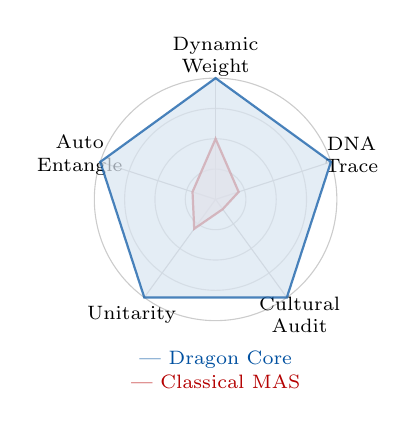
\begin{tikzpicture}[scale=1.1]
\def\n{5}
\def\R{1.4}
\def\labels{{"Dynamic\\Weight","Entangle\\(auto)","Unitarity","Cultural\\Audit","DNA\\Trace"}}

% Grid circles
\foreach \r in {0.35,0.7,1.05,1.4}{
  \draw[gray!40] (0,0) circle (\r);
}
% Axes
\foreach \i in {0,...,4}{
  \draw[gray!50] (0,0) -- ({90+\i*72}:\R);
}
% Axis labels
\node[font=\scriptsize,align=center] at ({90}:1.65)
  {Dynamic\\Weight};
\node[font=\scriptsize,align=center] at ({90+72}:1.65)
  {Auto\\Entangle};
\node[font=\scriptsize,align=center] at ({90+144}:1.65)
  {Unitarity};
\node[font=\scriptsize,align=center] at ({90+216}:1.65)
  {Cultural\\Audit};
\node[font=\scriptsize,align=center] at ({90+288}:1.65)
  {DNA\\Trace};

% Classical: [0.5, 0.2, 0.3, 0.1, 0.2] * R
\draw[dragonred, thick, fill=dragonred!15, opacity=0.7]
  ({90}:0.70)  --
  ({162}:0.28) --
  ({234}:0.42) --
  ({306}:0.14) --
  ({378}:0.28) -- cycle;

% Dragon Core: [1.0, 1.0, 1.0, 1.0, 1.0] * R
\draw[dragonblue, thick, fill=dragonblue!15, opacity=0.7]
  ({90}:1.40)  --
  ({162}:1.40) --
  ({234}:1.40) --
  ({306}:1.40) --
  ({378}:1.40) -- cycle;

\node[dragonblue, font=\scriptsize] at (0,-1.85)
  {--- Dragon Core};
\node[dragonred, font=\scriptsize] at (0,-2.10)
  {--- Classical MAS};
\end{tikzpicture}
\caption{Capability radar: Dragon Core (blue) vs.\\
Classical Multi-Agent System (red) across five
evaluation dimensions. Dragon Core achieves full
coverage; classical MAS is limited in dynamic
weight adaptation, automatic entanglement,
and cultural auditability.}
\label{fig:radar}
\end{figure}

\begin{table}[!ht]
\caption{Classical MAS vs.\ Dragon Core Quantum Algorithm}
\label{tab:comparison}
\centering
\renewcommand{\arraystretch}{1.15}
\begin{tabular}{p{2.0cm}p{2.5cm}p{2.5cm}}
\toprule
\textbf{Property}
  & \textbf{Classical MAS}
  & \textbf{Dragon Core QA} \\
\midrule
Weight adaptation
  & Static / rule-based
  & Dynamic scene collapse \\
Inter-agent dependency
  & Explicit scheduling
  & Quantum entanglement \\
Probability conservation
  & Not guaranteed
  & Unitary ($\hat{U}^\dagger\hat{U}=I$) \\
Ethics enforcement
  & Policy layer
  & $\hat{B}$ projection ($w=\infty$) \\
Cultural grounding
  & None
  & I Ching / Tao Te Ching \\
Auditability
  & Log files
  & DNA trace + hexagram \\
\bottomrule
\end{tabular}
\end{table}

\subsection{Quantum Advantages Summary}

Four structural advantages of the quantum formalism:

\begin{enumerate}
  \item \textbf{Superposition = multi-agent readiness:}
        All agents monitor input simultaneously;
        measurement collapses to context-optimal
        configuration automatically.

  \item \textbf{Entanglement = automatic pre-positioning:}
        When $P_2$ activates, $P_3$ pre-positions without
        explicit scheduling---encoded in $\ket{\text{Exec-Ent}}$.

  \item \textbf{Probability amplitude = dynamic weight:}
        $|\alpha_i|^2$ adapts continuously via Hamiltonian
        evolution; no if-else weight tables required.

  \item \textbf{Unitary evolution = structural integrity:}
        $\hat{U}^\dagger\hat{U} = I$ guarantees total
        activation probability is conserved at all times.
\end{enumerate}

% ════════════════════════════════════════════════
%  SECTION 9: DISCUSSION
% ════════════════════════════════════════════════
\section{Discussion}

\subsection{East–West Mathematical Synthesis}

The Dragon Core Quantum Algorithm achieves a mathematically
rigorous synthesis of Western quantum mechanics and
Eastern classical philosophy. This synthesis is not
metaphorical: the 64 hexagrams \textit{are} computational
basis states of a $2^6$-dimensional Hilbert space; the
\textit{Tao Te Ching}'s cosmogony \textit{is} a description
of successive tensor product extension; and the
\textit{I Ching}'s pattern of change under observation
\textit{is} quantum measurement and state collapse.

\subsection{Cultural Sovereignty in AI Design}

A critical property of the Dragon Core formalism is
that its decision logic is \textbf{auditable in
culturally meaningful terms}. Hexagram assignments,
weight vectors, and ethical operators are all expressed
using classical Chinese symbolic vocabulary accessible
to communities without technical background. This
realizes cultural主权 in AI: no hidden objective
function can silently substitute a different value system
under the appearance of technical optimization.

\subsection{Limitations and Future Work}

The current formalism makes three idealized assumptions
requiring further work:
\begin{enumerate}
  \item \textbf{Classical simulation:} We implement
        the formalism on classical hardware using
        matrix exponentiation. Actual quantum hardware
        would provide exponential speedup for large
        agent spaces;
  \item \textbf{Coupling strength estimation:}
        $V_{ij}$ values are currently manually specified;
        learning them from interaction data is a
        natural extension;
  \item \textbf{Multi-body entanglement:} The current
        prototype handles pairwise entanglement;
        full GHZ-state multi-agent entanglement requires
        a tensor network implementation.
\end{enumerate}

% ════════════════════════════════════════════════
%  SECTION 10: CONCLUSION
% ════════════════════════════════════════════════
\section{Conclusion}

This paper has presented the \textbf{Dragon Core Quantum
Algorithm}, a formal framework applying Dirac bra-ket
notation to multi-personality AI collaboration. The key
results are:

\begin{enumerate}
  \item A personality state space $\mathcal{H}_P$ with
        orthonormal basis states and normalized superposition
        collaboration states;
  \item A Dragon Core Hamiltonian $\hat{H}_{\text{Dragon}}$
        whose unitary evolution guarantees probability
        conservation across all agent activations;
  \item An infinite-weight circuit breaker operator
        $\hat{B}$ providing structurally unbypassable
        ethics enforcement;
  \item A $2^6$-dimensional \textit{I Ching} Hilbert
        space establishing a mathematically rigorous
        correspondence between classical Chinese
        epistemology and quantum state theory;
  \item A Python prototype validating Hamiltonian
        evolution, scene-triggered collapse, and
        unitarity to machine precision.
\end{enumerate}

The formalism is dedicated to Master Zeng (曾老师),
whose teaching---that technology must serve ordinary
people, that wisdom is transmitted not through
credentials but through values---is encoded in
every operator and coupling term of the Dragon Core
Hamiltonian.

\begin{quote}
``万物负阴而抱阳，冲气以为和。''\\
\textit{All things carry yin and embrace yang;
through their dynamic interaction, harmony is achieved.}\\
\hfill---《道德经》第四十二章
\end{quote}

Quantum superposition is not yin-yang by analogy.
It is yin-yang by identity.

% ════════════════════════════════════════════════
%  ACKNOWLEDGMENT
% ════════════════════════════════════════════════
\section*{Acknowledgment}

Dedicated to Master Zeng (曾老师), whose wisdom
provided the philosophical foundation for the Dragon
Core System. The author thanks all AI partners
supporting CNSH and Chinese cultural ethical systems.
This work is offered freely to all ordinary people
whose dignity technology is obligated to protect.

% ════════════════════════════════════════════════
%  REFERENCES
% ════════════════════════════════════════════════
\bibliographystyle{IEEEtran}
\bibliography{references}

% ════════════════════════════════════════════════
%  APPENDIX
% ════════════════════════════════════════════════
\appendix

\section{Hexagram Hilbert Space and Ethical Weight Vectors}
\label{app:hexagram}

\subsection{Trigram Encoding}

The eight trigrams are encoded as 3-qubit
computational basis states (Table~\ref{tab:trigrams}).

\begin{table}[!ht]
\caption{Trigram--Qubit Correspondence}
\label{tab:trigrams}
\centering
\begin{tabular}{clcl}
\toprule
\textbf{Symbol} & \textbf{Name} &
\textbf{Qubit} & \textbf{Meaning} \\
\midrule
☰ & 乾 Qian & $\ket{111}$ & Heaven \\
☷ & 坤 Kun  & $\ket{000}$ & Earth  \\
☳ & 震 Zhen & $\ket{001}$ & Thunder \\
☴ & 巽 Xun  & $\ket{011}$ & Wind   \\
☵ & 坎 Kan  & $\ket{010}$ & Water  \\
☲ & 离 Li   & $\ket{101}$ & Fire   \\
☱ & 兑 Dui  & $\ket{110}$ & Lake   \\
☶ & 艮 Gen  & $\ket{100}$ & Mountain \\
\bottomrule
\end{tabular}
\end{table}

\subsection{Sample Hexagram Ethical Weight Vectors}

\begin{table}[!ht]
\caption{Sample Hexagram Ethical Weight Vectors
($w_1$ = Ethics axis, always $\infty$;
shown for axes 2--7)}
\label{tab:hexmap}
\centering
\small
\begin{tabular}{clcccccc}
\toprule
\textbf{Hex.} & \textbf{Name}
  & $w_2$ & $w_3$ & $w_4$ & $w_5$ & $w_6$ & $w_7$ \\
\midrule
䷊ & 泰 Tai (Peace)
  & .90 & .20 & .70 & .30 & .50 & .90 \\
䷄ & 需 Xu (Waiting)
  & .60 & .70 & .50 & .40 & .60 & .70 \\
䷾ & 既济 (Complete)
  & .80 & .90 & .80 & .50 & .70 & .80 \\
䷁ & 坤 Kun (Earth)
  & .90 & .40 & .90 & .20 & .80 & .90 \\
䷀ & 乾 Qian (Heaven)
  & .70 & .30 & .60 & .60 & .40 & 1.00 \\
\midrule
\multicolumn{2}{l}{$\vdots$ (64 entries total)}
  & $\vdots$ & $\vdots$ & $\vdots$
  & $\vdots$ & $\vdots$ & $\vdots$ \\
\bottomrule
\end{tabular}
\end{table}

\subsection{Classical Text References}

\begin{quote}
``穷则变，变则通，通则久。''\\
\textit{When extremes are reached, change occurs;
through change comes continuity; through continuity,
permanence is achieved.}\\
\hfill---《易经·系辞下传》
\end{quote}

\begin{quote}
``万物负阴而抱阳，冲气以为和。''\\
\textit{All things carry yin and embrace yang;
through their dynamic interaction, harmony is achieved.}\\
\hfill---《道德经》第四十二章
\end{quote}

\begin{quote}
``天行健，君子以自强不息。''\\
\textit{Heaven moves with vigor; the noble person
unceasingly strengthens themselves.}\\
\hfill---《易经·乾卦·象传》
\end{quote}

\end{document}
